\chapter{METODOLOGIA}

Este capítulo apresenta a metodologia que foi utilizada ao longo do desenvolvimento de nossa pesquisa, e as justificativas para estas escolhas.

\section{Ferramenta de Simulação}

Durante nossa pesquisa bibliográfica, duas ferramentas de simulação compatíveis com o \emph{MapReduce} se destacaram, o MRPerf \cite{wang2009using} e o SLS \cite{ApacheSLS}. Avaliado a alguns anos em \cite{liu2013hsim}, o MRPerf possuí limitações para medir com precisão algumas etapas da estrutura do \emph{MapReduce}, especialmente nas fases de competição por recursos, tendo eficácia apenas na fase \emph{Shuffle}. Além disso, os benchmarks de TeraSort implementados pelos desenvolvedores do Hadoop e utilizados na validação do MRPerf em \cite{wang2009using} correspondem a versão do Hadoop 1.x, e, há claras diferenças entre as versões do Hadoop, que já foram apresentadas no tópico 2.5.4 do capítulo anterior.

Por outro lado, o SLS vem sendo utilizado constantemente em pesquisas de gerenciamento de filas no Hadoop, como em \cite{sharma2015performance} e \cite{shao2016energy}. Apesar de não ter sido desenvolvido originalmente para levar a rede em conta em suas simulações, recentemente o SLS foi estendido para NetSLS \cite{wette2015extending}, passando a integrar um módulo de rede \cite{wette2014maxinet}, que permite avaliar traços em tempo real da simulação.

O NetSLS \cite{wette2015extending} é uma ferramenta de simulação para avaliar ideias que, em conjunto, resolvem o problema de programação de trabalho e fluxo para aplicações de \emph{big data}. Esta ferramenta combina o \emph{Yarn Scheduler Load Simulator} \cite{ApacheSLS} com o emulador de rede distribuída MaxiNet \cite{wette2014maxinet}.

Com esta ferramenta, a interdependência entre a rede e as tarefas em execução nela podem ser incluídas na avaliação de novas ideias, aproveitando a pesquisa em aplicativos de \emph{big data} com programação conjunta de trabalho e fluxo de dados como demonstrado na figura 3.1.

\begin{figure}[htbp]
    \centering
    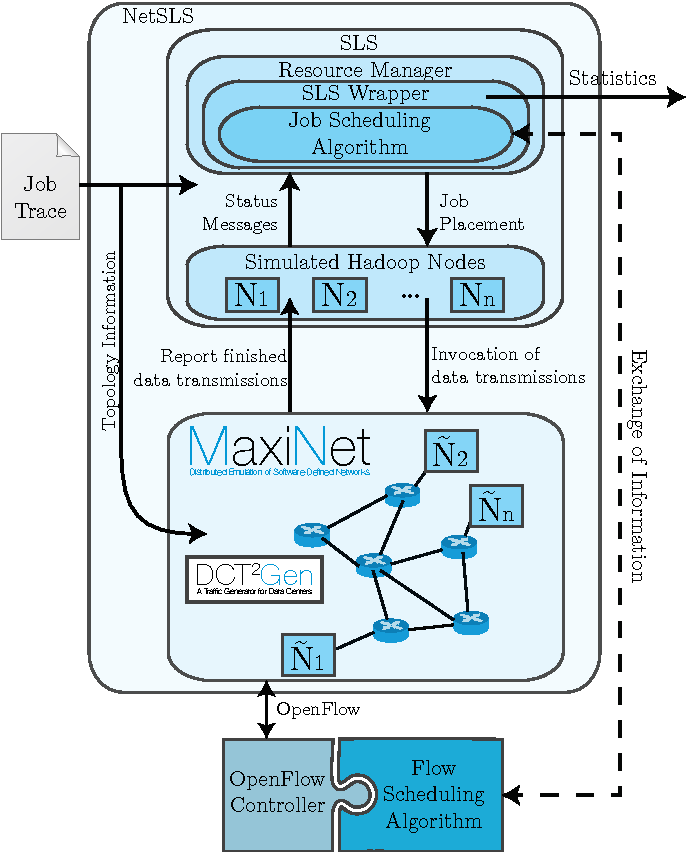
\includegraphics[width=9cm, height=11cm]{3-metodologia/Figura_2.jpg}
    \caption{Esquema do NetSLS sendo controlado por um OpenFlow externo}
    \cite{wette2015extending}
    \label{fig:NetSLS}
\end{figure}

Como ilustrado na figura 3.1, a extensão do SLS para NetSLS adiciona transmissões de dados reais às tarefas simuladas. No Hadoop, o processamento de uma tarefa consiste nas três fases sequenciais de busca de dados, processamento de dados e armazenamento de dados. Buscar e armazenar requer acesso aos dados. Dependendo da localização dos dados, isso envolve a rede. Para modelar a rede que interconecta os nós do Hadoop, o NetSLS usa o MaxiNet, um emulador de rede distribuída altamente realista para Redes Definidas por \emph{Software} (SDN). O MaxiNet distribui uma rede virtual em várias máquinas físicas (chamadas de \emph{workes}) tornando possível emular redes muito grandes (como as de \emph{datacenters}) em apenas alguns recursos físicos. Para distribuir um G{$_\mathit{V}$} de rede virtual que deve ser emulado em {$\mathit{n}$} \emph{workers}, o MaxiNet primeiro divide o G{$_\mathit{V}$} em {$\mathit{n}$} partes. Em seguida, cada partição é emulada em cada um dos \emph{workers}. Todo o tráfego entre as diferentes partições é canalizado por meio da rede física que interconecta os \emph{workes} na partição de destino. Na inicialização, o NetSLS busca a topologia do \emph{cluster} de um arquivo complementar ao rastreamento do trabalho e configura o MaxiNet para emular a rede. Para cada nó N{$_\mathit{i}$} simulado do Hadoop, o NetSLS emula um nó correspondente, Ñ{$_\mathit{i}$} usando MaxiNet. Sempre que o planejador decide executar uma tarefa no N{$_\mathit{i}$}, o NetSLS procura informações sobre as transferências de dados do rastreamento do trabalho e inicia as transferências correspondentes em Ñ{$_\mathit{i}$}. A conclusão da transferência é subsequentemente relatada de Ñ{$_\mathit{i}$} para N{$_\mathit{i}$} que, por sua vez, relata uma conclusão bem-sucedida ao planejador de trabalho quando as três fases do trabalho terminam \cite{wette2015extending}.

Como o MaxiNet emula um SDN compatível com \emph{OpenFlow}, um controlador \emph{OpenFlow} gerencia a rede. O \emph{OpenFlow} é um protocolo de comunicação baseado em um \emph{switch Ethernet}, com uma tabela de fluxo interna e uma interface padronizada para adicionar e remover entradas de fluxo \cite{mckeown2008openflow}. Um administrador de rede pode particionar o tráfego em fluxos de produção e pesquisa. Os pesquisadores podem controlar seus próprios fluxos - escolhendo as rotas que seus pacotes seguem e o processamento que recebem. Dessa forma, é possível experimentar novos protocolos de roteamento, modelos de segurança, esquemas de endereçamento e até alternativas ao IP \cite{mckeown2008openflow}.

O controlador é externo ao NetSLS, portanto, qualquer controlador \emph{OpenFlow} pode ser usado para controlar o comportamento da rede. O planejador de fluxo reside no controlador \emph{OpenFlow}. Por fazer parte do controlador, ele tem acesso a todas as informações presentes no controlador. Para trocar informações com o planejador de trabalho, uma interface personalizada entre o planejador de trabalho e fluxo pode ser estabelecida. Para avaliar novas ideias sob diferentes cargas de rede, ao NetSLS também foi integrado o DCT²Gen \cite{wette2014dct}, um gerador de tráfego para tráfego de \emph{data center} altamente realista. No NetSLS, o DCT²Gen cria tráfego de segundo plano, imitando o tráfego cruzado de outras aplicações.

Ao transformar o SLS em NetSLS, tem-se a oportunidade de testar novos algoritmos de agendamento de trabalho e fluxo. Ao longo do rastreamento de trabalho e uma descrição de topologia, as únicas duas entradas para NetSLS são um algoritmo de agendamento de trabalho e um controlador \emph{OpenFlow} implementando o algoritmo de agendamento de fluxo desejado. O NetSLS irá então simular a interação entre o fluxo e o planejador de trabalho no rastreamento do trabalho, levando a uma avaliação rápida e realista de novos algoritmos de planejamento sem exigir um teste caro ou uma simulação personalizada \cite{wette2015extending}.

Diante dessas avalições, optamos para nossa pesquisa a utilização do NetSLS para avaliar o impacto do EEE no Hadoop em relação à economia de energia e desempenho. O NetSLS é o SLS estendido com um modelo realista de rede e tráfego, o MaxiNet. Para poder simular conexões EEE, o NetSLS foi amplificado com um modelo realista \cite{reviriego2011using}. Essa metodologia nos permitiu ter uma visão ampla da execução com traços em \emph{logs}, e assim calcular a economia de energia e o desempenho.

\section{Topologia}

A topologia do \emph{cluster} escolhida para este trabalho foi a \emph{Leaf-Spine} \cite{CiscoLeafSpine}, como pode ser observado na Figura 3.1. A escolha desta topologia se dá ao fato da arquitetura \emph{Leaf-Spine} ser recomendada para computadores de escala \emph{Warehouse} \cite{efficiency2012cisco} quando concentrados em tráfego leste-oeste entre servidores do mesmo \emph{cluster} \cite{IntroductionLeafSpine}. 


A topologia \emph{Leaf-Spine} traz \emph{Switches} de \emph{Spine} e \emph{Leafs} que são semelhantes aos \emph{Switches} de acesso e agregação encontrados na clássica \emph{K-ary Fat Tree} \cite{vahdat2013scalable}. A vantagem da topologia \emph{Leaf-Spine} quando comparada com a \emph{K-ary Fat Tree} é sua conectividade de malha completa entre \emph{Switches} de \emph{Leafs} e \emph{Spine}, mas segue de fato uma arquitetura \emph{Two-Tier Clos}. Cada \emph{Switch} em \emph{Leaf}, também conhecido como \emph{Switch Top of Rack} (ToR), é conectado ao \emph{Switch} de \emph{Spine}, denominado \emph{Switch} de Agregação regularmente no modelo de \emph{Fat Tree}, usando um único link. A \emph{Leaf-Spine} pode `expandir-se' para um número razoavelmente grande de servidores simplesmente adicionando mais \emph{Switches}, embora isso também aumente a quantidade de cabos e os custos dos equipamentos de rede necessários, uma vez que cada \emph{Leaf Switch} deve ser conectado a cada \emph{Spine Switch} \cite{IntroductionLeafSpine}.

\begin{figure}[htp]
    \centering
    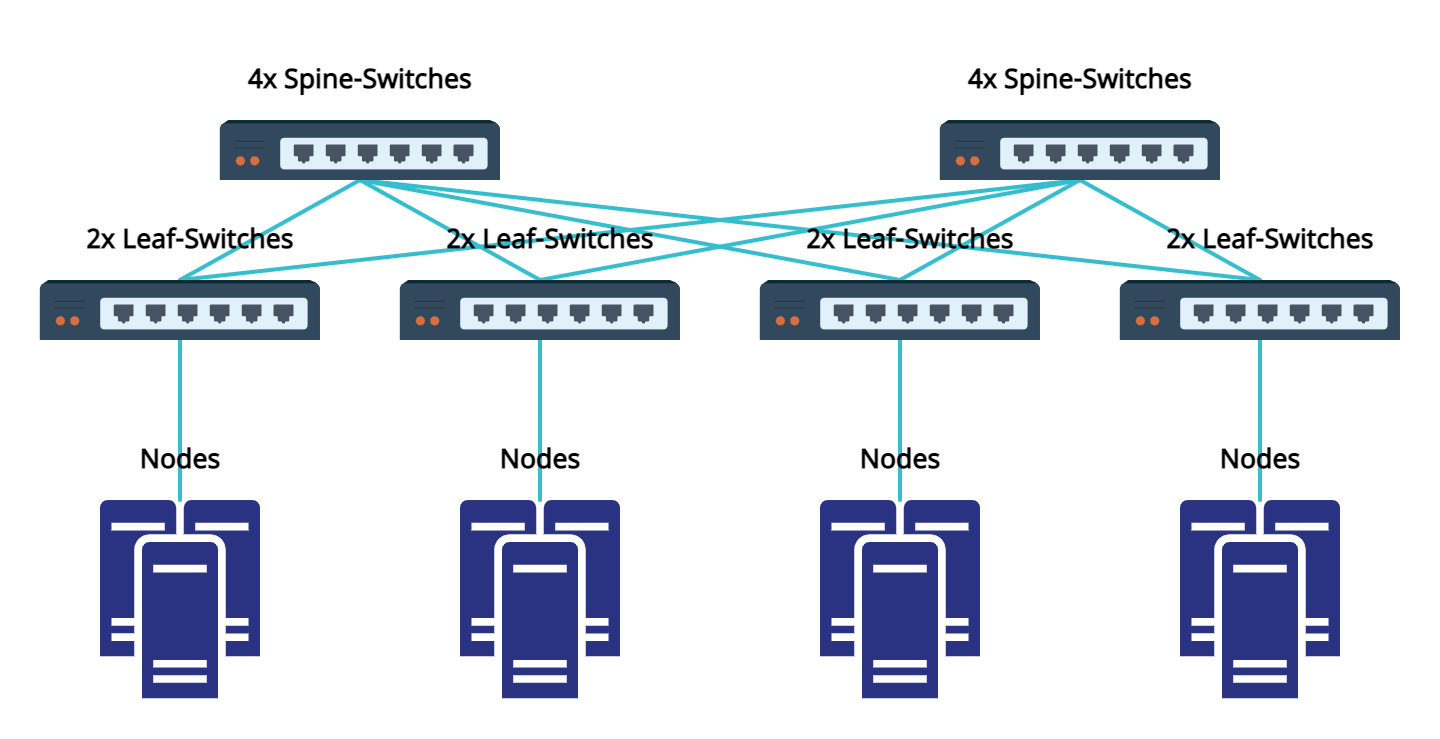
\includegraphics[width=14cm]{3-metodologia/Topologia de Rede - Dissertação.png}
    \caption{Topologia de Rede Leaf-Spine}
    \cite{CiscoLeafSpine}
    \label{fig:TopologiaDeRede}
\end{figure}


É importante mencionar que a topologia da \emph{Leaf-Spine} pode ser categorizada como uma topologia de \emph{Fat Tree} de dois níveis, ou seja, sem a camada de agregação entre a borda e a camada central, e não está organizada em \emph{Pods} \cite{FatTreeDesign}; \cite{testa2017optical}. Como o foco de nossa pesquisa foi analisar as configurações do E-EON \cite{silva2018eon} sobre a atual versão do Hadoop \emph{MapReduce}, decidimos considerar a mesma topologia \emph{Leaf-Spine} para esta pesquisa, que também é recomendada para o Hadoop, como visto em várias referências de \emph{design} de \emph{clusters} \cite{bechtolsheim2011big}; \cite{efficiency2012cisco}; \cite{BigDataGuide}.

\begin{table}[!htp]
\centering
\caption{Topologia Simulada}
\label{Topologia Simulada}
\def\arraystretch{1.2}
\begin{tabular}{c c c}
\hline
Categoria & Parâmetro & Valor \\
\hline
Cluster & Nodes & 60, 96, 100, 150,\\
 & & 160, 240, 250, 256,\\
 & & 400 ou 640\\
 & Number of racks & 4\\
Network & Each node & 1GbE/10GbE/25GbE\\
 & & 40GbE : 1\\
 & & ---\\
 & Each leaf switch & 1GbE/10GbE/25GbE\\
 & & 40GbE : 15, 24, 25,\\
 & & 37, 38, 40, 60, 62, 63\\
 & & 64, 100 ou 160\\
 & & 10GbE/25GbE/40GbE\\
 & & 100GbE/400GbE: 2\\
 & Each spine switch & ---\\
 & & 10GbE/25GbE/40GbE\\
 & & 100GbE/400GbE: 4\\
\hline
\end{tabular}
\end{table}

A Tabela 3.1 detalha a topologia de rede simulada. Simulamos vários \emph{clusters} de 60, 96, 100, 150, 160, 240, 250, 256, 400 e 640 nodos divididos em 4 \emph{racks}, cada nodo com um \emph{Intel Xeon 2.13GHz E5506 quad-core} e um único link no \emph{top-of-rack} (ToR), que varia entre 1GbE, 10GbE, 25GbE ou 40GbE. Cada \emph{switch top-of-rack} é conectado a um \emph{switch} de agregação usando um único link de 10GbE, 25GbE, 40GbE, 100GbE ou 400GbE, dependendo da simulação. As taxas de excesso de assinatura (\emph{oversubscription ratio}) em nossos testes foram de 1.5:1, 2.5:1 e 4:1, o que corresponde à recomendação da Cisco para implantação do \emph{MapReduce} com uma taxa de excesso de assinatura de 4:1 ou menor na camada de acesso \cite{Cisco2011TechReport}. Segundo \cite{Clusterplaningguide}, ter um baixo índice de excesso de assinatura é uma forma de melhorar o desempenho da rede com investimentos em equipamentos.

%Table  I  details  the  simulated  scenario.  We  simulated  multiple  clusters  of  60,  96,  100,  150,  160,  240,  250,  256,  400,and 640 nodes, each node having a quad-core Intel Xeon 2.13GHz E5506 and a single link on the top-of-rack (ToR), whichvaries  between  1GbE,  10GbE,  25GbE  or  40GbE.  Each  top-of-rack switch is connected to an aggregation switch using asingle  link  of  10GbE,  25GbE,  40GbE,  100GbE  or  400GbE,depending  on  the  simulation.  The  oversubscription  ratios  inour  tests  were  1.5:1,  2.5:1,  and  4:1,  which  corresponds  toCisco’s  recommendation  to  MapReduce  deployment  with  anoversubscription ratio of 4:1 or less at the access layer [28]. Asstated by [29], having an low oversubscription ratio is a way toimprove network performance with investments in equipment.

\section{Consumo de Energia dos Switches}

Um dos aspectos mais importantes desta pesquisa foi a definição do consumo de energia das redes simuladas, dando assim uma base de cálculo correta. Para isso, foi realizada uma pesquisa à procura dos switches que são optados pelas indústrias em produção. Por ter um guia completo disponível com todas as informações necessárias para nossa pesquisa e ser um produto padrão do mercado, optamos pela escolha da Série Juniper QFX5220 \cite{QFX5220Guide}.

Na tabela 3.2 é possível observar as configurações padrões dos \emph{Switches} desta linha, em que temos 64 \emph{megabytes} de \emph{buffers} distribuídos entre as portas, além de um consumo de 0.5w/h para links ethernet de 1Gb; 2.68w/h para 10Gb; 5.41w/h para 25Gb; 10.89w/h para 100Gb e 22.21/wh para 400Gb. 

\begin{table}[!htp]
\centering
\caption{Configuração dos Switches}
\label{Configuração dos Switches}
\def\arraystretch{1.2}
\begin{tabular}{c c c}
\hline
Categoria & Parâmetro & Valor \\
\hline
Buffers & Juniper QFX5220 & Total packet 64Mb\\
Link Power & 1GbE & 0.5w/h\\
 & 10GbE & 2.68w/h\\
 & 25GbE & 5.41w/h\\
 & 40GbE & 7.49w/h\\
 & 100GbE & 10.89w/h\\
 & 400GbE & 22.21w/h\\
\hline
\end{tabular}
\end{table}

\section{Configurações do Cluster Hadoop}

Reservamos um nodo de um dos \emph{racks} do \emph{cluster} para execução do \emph{JobTracker}, enquanto 56, 92, 96, 146, 156, 236, 246, 252, 396 ou 636 nodos são reservados para execução das tarefas \emph{Map} e \emph{Reduce}. Além disso, cada um dos 3 \emph{racks} restantes executa 1 \emph{Namenode}, totalizando 3, que é a recomendação da Apache, oferecendo assim um equilíbrio entre escalabilidade e sobrecarga de comunicação \cite{HDFSHighAvailability}.

\begin{table}[!htp]~
\centering
\caption{Configurações do Cluster Hadoop}
\label{Simulation_Environment}
\def\arraystretch{1.2}
\begin{tabular}{c c c}
\hline
Categoria & Parâmetro & Valor \\
\hline
Sistema & Nodes & 60, 96, 100, 150,\\
 & & 160, 240, 250, 256,\\
 & & 400 ou 640\\
 & Racks & 4\\
Config. & Jobtracker & 1\\
 & Namenodes & 3\\
 & Workers & 56, 92, 96, 146,\\
 & & 156, 236, 246, 252,\\
 & & 396 ou 636\\
 & Scheduler Scheme & Fair\\
TCP buffer & Default size & 128 KB por conexão\\
TCP packet & Default size & 1500 bytes\\
\hline
\end{tabular}
\end{table}


\section{Configurações do Energy Efficient Ethernet}


Para as operações de \emph{wake} e \emph{sleep} do EEE assumimos os valores disponíveis na Tabela 3.4 fornecida por \cite{reviriego2009performance} e \cite{6891095}, e na Tabela 3.5. Para links de 40GbE e 100GbE, usamos os valores dos modos \emph{Deep Sleep} e {Fast Wake} \cite {6891095}, disponíveis nas tabelas 3.4 e 3.6 respectivamente.

\begin{table}[!htp]
\centering
\caption{EEE - Tempo das operações \emph{wake} e \emph{sleep} no modo \emph{Deep Sleep}}
\label{EEE wake and sleep operations times}
\def\arraystretch{1.2}
\begin{tabular}{c c c}
\hline
PHY & Min. \emph{Tw} (µs) &  Min. \emph{Ts} (µs)\\
\hline
1000Base-T & 16,5 & 182\\
10GBase-T & 4,48 & 2,88\\
40GBase & 5,5 & 0,9\\
100GBase & 5,5 & 0,9\\
\hline
\end{tabular}
\end{table}

Como não há projetos ou pesquisas para implementações do Energy Efficient Ethernet em links de 25GbE e 400GbE, os valores do Min.$T_w$ e  Min.$T_s$ não estão disponíveis em nenhuma fonte confiável conhecida. Assim, calculamos os valores médios para 25GbE dos links de 10GbE e 40GbE; por outro lado, para o link de 400GbE, assumimos os mesmos valores dos links de 100GbE fornecidos por \cite{6891095}, uma vez que o projeto se assemelha.

%As there are no projects or researches for implementations of Energy Efficient Ethernet in 25GbE and 400GbE links, the Min. $T_w$ and  Min. $T_s$ values are not available from any known trusted source. Thus, we calculated the average values for 25GbE from the 10GbE and 40GbE links; on the other hand, for the 400GbE link, we used same values of 100GbE links provided by \cite {b32}.

\begin{table}[!htp]
\centering
\caption{EEE - Tempos assumidos para as operações \emph{wake} e \emph{sleep} no modo \emph{Deep Sleep}}
\label{Generated EEE wake and sleep operations times}
\def\arraystretch{1.2}
\begin{tabular}{c c c}
\hline
PHY & Min. \emph{Tw} (µs) &  Min. \emph{Ts} (µs)\\
\hline
25GBase & 4,99 & 1,89\\
400GBase & 5,5 & 0,9\\
\hline
\end{tabular}
\end{table}

\begin{table}[!htp]
\centering
\caption{EEE - Tempo das operações \emph{wake} e \emph{sleep} no modo \emph{Fast Wake}}
\label{EEE wake and sleep operations times on Fast Wake Mode}
\def\arraystretch{1.2}
\begin{tabular}{c c c}
\hline
PHY & Min. \emph{Tw} (µs) &  Min. \emph{Ts} (µs)\\
\hline
40GBase & 0,34 & 0,25\\
100GBase & 0,34 & 0,25\\
\hline
\end{tabular}
\end{table}

\section{Configurações do Packet Coalescing}

De acordo com \cite{herreri2012optimal}, configurar o \emph{Packet Coalescing} da forma correta é o ponto chave crítico para economia de energia e performance adequadas. Nossas configurações vem de artigos publicados ao longo de pesquisas que envolvem \emph{Packet Coalescing} e \emph{Energy Efficient Ethernet}, como 12$\mu$s10 e 120$\mu$s100 de \cite{christensen2010ieee}, 500$\mu$s500 de \cite{silva2018eon} e 1ms1000 de \cite{reviriego2010burst}. Configurações com tempo de espera acima de 10ms não foram consideradas, pois, degradam drasticamente o desempenho do \emph{MapReduce} \cite {silva2018eon}.

\begin{table}[!htp]
\centering
\caption{Configurações do \emph{Packet Coalescing}}
\label{Configurações do Packet Coalescing}
\def\arraystretch{1.2}
\begin{tabular}{c c c}
\hline
Label & Tempo de Espera & Gatilho\\
\hline
12µs10   & 12µs  & 10 pacotes\\
120µs100 & 120µs & 100 pacotes\\
500µs500 & 500µs & 500 pacotes\\
1ms1000  & 1ms   & 1000 pacotes\\
\hline
\end{tabular}
\end{table}

\section{Configurações do Active Queue Management e Explicit Congestion Notification}

Para a utilização da \emph{Active Queue Management} escolhemos dois algoritmos, o \emph{Random Early Detection} e o \emph{Controlled Delay}.

\begin{table}[!htp]
\centering
\caption{Valores definidos {$\mathit{Min}_\mathit{th}$} e {$\mathit{Max}_\mathit{th}$} para o \emph{Random Early Detection}}
\label{Valores definidos para o RED}
\def\arraystretch{1.2}
\begin{tabular}{c c c}
\hline
\emph{Label} & {$\mathit{Min}_\mathit{th}$} & {$\mathit{Max}_\mathit{th}$}\\
\hline
Min70Max70 & 70  & 70\\
Min125Max375 & 125  & 375\\
Min25Max75 & 25  & 75\\
Min50Max150 & 50  & 150\\
\hline
\end{tabular}
\end{table}

O primeiro, RED, é normalmente implementado usando o AQL (\emph{Average Queue Length}) para decisões de marcação ou descarte de pacotes, entretanto, usamos o IQL (\emph{Instant Queue Length}), pois trabalhos anteriores já demonstraram que se encaixa melhor em redes de alta velocidade como em \emph{data centers} \cite{alizadeh2010data}; \cite {silva2018eon}. Por fim, definimos os valores demonstrados na tabela 3.8 baseados em trabalhos anteriores, como 70 {$\mathit{Min}_\mathit{th}$} e 70 {$\mathit{Max}_\mathit{th}$}  em \cite{alizadeh2010data}; 125 {$\mathit{Min}_\mathit{th}$} e 375 {$\mathit{Max}_\mathit{th}$}, 25 {$\mathit{Min}_\mathit{th}$} e 75 {$\mathit{Max}_\mathit{th}$}, 50 {$\mathit{Min}_\mathit{th}$} e 150 {$\mathit{Max}_\mathit{th}$} em \cite{silva2018eon}.

O segundo, CoDel, usamos a implementação \emph{default} sem nenhuma modificação. O CoDel é considerado uma fila sem parâmetros, mas o administrador da rede ainda precisa fornecer dois valores, atraso de destino (\emph{target delay}) e intervalo (\emph{interval}).

\begin{table}[!htp]
\centering
\caption{Valores definidos para o \emph{Controlled Delay}}
\label{Valores definidos para o CoDel}
\def\arraystretch{1.2}
\begin{tabular}{c c c}
\hline
\emph{Label} & \emph{Target delay} & \emph{Interval}\\
\hline
500µs20ms & 500µs  & 20ms\\
300µs0.75µs & 300µs  & 0.75µs\\
400µs1ms & 400µs  & 1ms\\
800µs1.5ms & 800µs  & 1.5ms\\
\hline
\end{tabular}
\end{table}

Os valores assumidos para o CoDel foram de: 500$\mu$s para \emph{target delay} e 20ms para \emph{interval} fornecidos por \cite{bufferbloat}; 300$\mu$s para \emph{target delay} e 0.75$\mu$s para \emph{interval} fornecidos por \cite{ismaileffectiveness}; 400$\mu$s e 800$\mu$s para \emph{target delay}, 1ms e 1.5ms para \emph{interval} fornecidos por \cite{silva2018eon}; e estão expostos na tabela 3.9.

Por fim, utilizamos a configuração \emph{deafult} do \emph{Explicit Congestion Notification} considerando uma implementação real (nos \emph{switches}) - nesta configuração pacotes ECT-capable, SYN, SYN-ACK e ACKs que possuam o ECE-bit não são descartados antecipadamente.

\section{Cargas de Trabalho}

%We chose two workloads, small tasks and batch. The small workload consists of a sequence of small jobs, each with ten map tasks and one reduce task. We force an average CPU utilization about to 40\%, which is compatible with a study of traces obtained at Facebook. The batch workload is closer to batch processing for real big data applications, and we involve the entire system using a single large job, with the number of map and reduce tasks both equal to twice the number of worker nodes.

Para os testes de nossa pesquisa foram definidas duas cargas de trabalho, \emph{small tasks} e {batch}. A \emph{small tasks} consiste em uma sequência de pequenos trabalhos, cada um com dez tarefas de mapeamento (\emph{map}) e uma tarefa de redução (\emph{reduce}). Forçamos uma utilização média do CPU em torno de 40\%, o que é compatível com um estudo de traços obtido no Facebook \cite{chen2011case}.
 
\begin{table}[!htp]
\centering
\caption{Cargas de Trabalho Simuladas}
\label{Cargas de Trabalho Simuladas}
\def\arraystretch{1.2}
\begin{tabular}{c c c}
\hline
Categoria & Parâmetro & Valor \\
\hline
Jobs & Maps & Small jobs: 10\\
 & & Batch jobs: 2\\
 & Reduces & Small jobs: 1\\
 & & Batch jobs: 2\\
\hline
\end{tabular}
\end{table}

Quanto ao \emph{batch}, a carga de trabalho foi semelhante ao processamento em lote para aplicativos de \emph{big data} reais \cite{chen2012interactive}, e envolvemos todo o sistema usando um único \emph{job} grande, com o número de tarefas de mapeamento (\emph{map}) e redução (\emph{reduce}) igual ao dobro do número de nodos de trabalho.

\section{Ciclo de Testes}

Para nosso ciclo de testes foi definido uma metodologia baseada na média aritmética \ref{eq:arithmeticmean} \cite{plackett1958studies} e desvio padrão \ref{eq:standard_deviation} \cite{brenner1988simple}.

\begin{equation}
\centering
{\displaystyle A={\frac {1}{n}}\sum _{i=1}^{n}a_{i}={\frac {a_{1}+a_{2}+\cdots +a_{n}}{n}}}
\label{eq:arithmeticmean}
\end{equation}

\begin{equation}
\centering
s = \sqrt{\frac{1}{N-1} \sum_{i=1}^N (x_i - \overline{x})^2}
\label{eq:standard_deviation}
\end{equation}

Primeiro é realizado cinco testes e calculado o desvio padrão dos mesmos. Os novos testes são interrompidos quando um novo teste está dentro da média dos testes anteriores acrescida ou subtraída do desvio padrão. Então é calculado a média dos testes anteriores juntamente ao novo teste, e por fim anotado o resultado final da simulação.

\begin{equation}
\centering
nT \leq A+s \quad \textrm{ou} \quad nT \geq A-s
\label{eq:finalequation}
\end{equation}

Pode-se observar de forma clara na fórmula \ref{eq:finalequation}, em que \textbf{`nT'} significa novo teste, \textbf{`A'} corresponde a média aritmética e \textbf{`s'} ao desvio padrão. Desta forma atingimos uma confiabilidade dos resultados de 95\% \cite{peck2015introduction}.

\section{Considerações Finais}

Neste capítulo foram apresentados as escolhas de configurações para o desenvolvimento da pesquisa. Primeiramente nossa ferramenta de simulação, o NetSLS \cite{wette2015extending}, uma extenção do \emph{YARN Scheduler Load Simulator} \cite{ApacheSLS}, em que torna-se possível a simulação de \emph{clusters} Hadoop \emph{MapReduce} em máquinas convencionais, facilitando assim o teste de protocolos de rede e esquemas de gerenciamento de fila.

Em seguida, definimos a topologia \emph{Leaf-Spine} \cite{CiscoLeafSpine} baseada em trabalhos anteriores sobre máquinas de escala \emph{Warehouse} concentradas em tráfego leste-oeste entre servidores do mesmo \emph{cluster} \cite{efficiency2012cisco}; \cite{IntroductionLeafSpine}. Quanto ao consumo de energia dos \emph{switches}, por ser um produto padrão do mercado, optamos pela escolha da Série Juniper QFX5220 \cite{QFX5220Guide}. O \emph{cluster} Hadoop foi configurado de acordo com as recomendações da Apache \cite{HDFSHighAvailability}, oferecendo assim um equilíbrio entre escalabilidade e sobrecarga de comunicação.

Para as conexões Ethernet escolhemos utililzar \emph{Active Queue Managements} como \emph{Controlled Delay} e \emph{Random Early Detection} com \emph{Explicit Congestion Notification} juntamente ao \emph{Energy Efficient Ethernet}, com o objetivo de procurar as melhoreres combinações e configurações dentre as disponíveis \cite{alizadeh2010data}; \cite{christensen2010ieee}; \cite{bufferbloat}; \cite{ismaileffectiveness}; \cite{reviriego2010burst}; \cite{silva2018eon} para as conexões de 1GbE, 10GbE, 25GbE, 40GbE, 100GbE e 100GbE. Por fim, aplicamos cargas de trabalhos \emph{small tasks} e \emph{batch} semelhantes à aplicativos de \emph{big data} reais \cite{chen2011case}; \cite{chen2012interactive}, e definimos um ciclo de testes baseado na média aritmética \ref{eq:arithmeticmean} \cite{plackett1958studies} e desvio padrão \ref{eq:standard_deviation} \cite{brenner1988simple} que proporciona uma confiabiliade dos resultados de 95\% \cite{peck2015introduction}.